

% ==========================================================
\section*{Learning Objectives -- Mục tiêu bài học}
\addcontentsline{toc}{section}{Mục tiêu bài học}

Bài ANN8 tiếp tục nội dung về underfitting và overfitting, nhưng tập trung hơn vào nguyên nhân và các kỹ thuật xử lý. Sau khi học xong, người học cần nắm được:

\begin{enumerate}[label=\arabic*.]
    \item Nhắc lại ý nghĩa của underfitting và overfitting trong bài toán phân loại và hồi quy.
    \item Hiểu nguyên nhân gây underfitting: mô hình quá đơn giản hoặc huấn luyện chưa đủ.
    \item Hiểu nguyên nhân gây overfitting: mô hình quá phức tạp, dữ liệu ít hoặc dữ liệu thiếu đa dạng.
    \item Biết một số hướng xử lý underfitting.
    \item Biết một số hướng xử lý overfitting: đơn giản hóa mô hình, bỏ bớt đặc trưng, tăng dữ liệu, data augmentation, early stopping và dropout.
    \item Hiểu ý nghĩa của train/validation/test set và nguyên tắc sử dụng từng tập.
    \item Hiểu vì sao dùng sai tập test có thể làm sai lệch kết quả nghiên cứu.
    \item Nắm được trực giác của dropout: không cho mạng phụ thuộc quá mạnh vào một số neuron cụ thể.
\end{enumerate}

% ==========================================================
\section{Underfitting \& Overfitting Recap -- Ôn lại Underfitting và Overfitting}

\subsection{Underfitting}

Underfitting là tình huống mô hình chưa khớp được với dữ liệu. Nói cách khác, mô hình chưa học được xu hướng tổng quát của dữ liệu.

Thường gặp khi:

\begin{itemize}
    \item mô hình quá đơn giản;
    \item số tham số quá ít;
    \item kiến trúc mạng quá yếu;
    \item thời gian huấn luyện chưa đủ;
    \item đặc trưng đầu vào chưa đủ thông tin.
\end{itemize}

\begin{ghinho}
Underfitting nghĩa là mô hình chưa đủ khả năng học bài toán. Dù có tiếp tục dùng mô hình quá đơn giản, sai số vẫn có thể không giảm đến mức mong muốn.
\end{ghinho}

\subsection{Overfitting}

Overfitting là tình huống mô hình quá khớp với dữ liệu huấn luyện. Khi đó, sai số trên tập huấn luyện có thể rất thấp, thậm chí gần bằng 0, nhưng mô hình lại làm việc kém trên dữ liệu mới.

Thường gặp khi:

\begin{itemize}
    \item mô hình quá phức tạp so với bài toán;
    \item dữ liệu huấn luyện quá ít;
    \item dữ liệu thiếu đa dạng;
    \item mô hình học cả nhiễu và chi tiết bất thường;
    \item quá trình huấn luyện kéo dài quá lâu.
\end{itemize}

\begin{canhbao}
Overfitting nguy hiểm hơn underfitting ở chỗ: trên tập huấn luyện, mô hình có vẻ rất tốt vì loss thấp. Nếu không kiểm tra đúng cách, ta có thể nhầm rằng mô hình đã làm việc tốt.
\end{canhbao}

\subsection{So sánh ngắn gọn}

\begin{center}
\begin{tabular}{p{0.24\textwidth}p{0.34\textwidth}p{0.32\textwidth}}
\toprule
Trường hợp & Biểu hiện & Nguyên nhân thường gặp \\
\midrule
Underfitting & Sai nhiều trên cả train và test & Mô hình quá đơn giản hoặc train chưa đủ \\
Good fitting & Học được xu hướng chung, test tốt & Mô hình phù hợp với độ phức tạp bài toán \\
Overfitting & Train rất tốt, test kém & Mô hình quá phức tạp hoặc dữ liệu ít/thiếu đa dạng \\
\bottomrule
\end{tabular}
\end{center}

% ==========================================================
\section{Underfitting \& Overfitting: Classification -- Ví dụ Underfitting và Overfitting trong phân loại}

\subsection{Mô tả bài toán phân loại}

Giả sử ta có dữ liệu 2D, ví dụ:

\[
    x_1 = \text{chiều cao}, \qquad x_2 = \text{cân nặng}
\]

Mỗi điểm dữ liệu thuộc một trong hai class:

\[
    C_1 \quad \text{hoặc} \quad C_2
\]

Mục tiêu là tìm một đường ranh giới để phân biệt hai class.

\subsection{Underfitting trong phân loại}

Nếu ranh giới thật cần là một đường cong, nhưng ta chỉ dùng một đường thẳng, mô hình có thể không phân chia tốt hai class.

\begin{center}
\begin{tikzpicture}[scale=0.9,>=Stealth]
    \draw[->] (0,0) -- (5,0) node[right] {$x_1$};
    \draw[->] (0,0) -- (0,4) node[above] {$x_2$};

    % Class 1
    \foreach \x/\y in {0.8/0.7,1.2/1.0,1.5/1.4,2.0/1.8,2.5/2.1,3.0/2.3}
        \draw[blue,thick] (\x,\y) circle (2pt);

    % Class 2
    \foreach \x/\y in {1.0/3.1,1.5/3.2,2.1/3.0,2.7/2.85,3.3/2.65,3.9/2.45}
        \draw[red,thick] (\x-0.06,\y-0.06) -- (\x+0.06,\y+0.06)
                          (\x-0.06,\y+0.06) -- (\x+0.06,\y-0.06);

    % Underfit boundary
    \draw[thick,orange] (0.5,2.0) -- (4.5,1.75);
    \node[orange] at (3.6,0.8) {Đường thẳng quá đơn giản};

\end{tikzpicture}
\end{center}

\begin{vidu}
Nếu dữ liệu có xu hướng cong nhưng mô hình chỉ có khả năng tạo đường thẳng, ta xoay hoặc dịch đường thẳng thế nào cũng khó phân loại tốt. Đây là ví dụ điển hình của underfitting.
\end{vidu}

\subsection{Overfitting trong phân loại}

Ngược lại, nếu mô hình quá mạnh, nó có thể tạo ra một đường ranh giới rất ngoằn ngoèo để phân loại đúng mọi điểm huấn luyện, kể cả các điểm nhiễu.

\begin{center}
\begin{tikzpicture}[scale=0.9,>=Stealth]
    \draw[->] (0,0) -- (5,0) node[right] {$x_1$};
    \draw[->] (0,0) -- (0,4) node[above] {$x_2$};

    % Class 1
    \foreach \x/\y in {0.8/0.7,1.2/1.0,1.5/1.4,2.0/1.8,2.5/2.1,3.0/2.3,3.5/2.85}
        \draw[blue,thick] (\x,\y) circle (2pt);

    % Class 2
    \foreach \x/\y in {1.0/3.1,1.5/3.2,2.1/3.0,2.7/2.85,3.3/2.65,3.9/2.45}
        \draw[red,thick] (\x-0.06,\y-0.06) -- (\x+0.06,\y+0.06)
                          (\x-0.06,\y+0.06) -- (\x+0.06,\y-0.06);

    % Overfit boundary
    \draw[thick,orange,smooth] plot coordinates {
        (0.6,2.25) (1.1,2.35) (1.6,2.50) (2.1,2.43)
        (2.6,2.62) (3.05,2.48) (3.35,3.12) (3.75,2.68) (4.3,2.85)
    };
    \node[orange] at (3.5,0.8) {Ranh giới quá phức tạp};

\end{tikzpicture}
\end{center}

\begin{ghinho}
Overfitting trong phân loại thường biểu hiện bằng ranh giới quyết định quá phức tạp, cố gắng ``né'' từng điểm dữ liệu thay vì học xu hướng chung.
\end{ghinho}

% ==========================================================
\section{Underfitting \& Overfitting: Regression -- Ví dụ Underfitting và Overfitting trong hồi quy}

\subsection{Mô tả bài toán hồi quy}

Hồi quy là bài toán dự đoán giá trị liên tục.

Ví dụ:

\begin{itemize}
    \item sản lượng điện tiêu thụ trong ngày;
    \item giá nhà;
    \item nhiệt độ ngày mai;
    \item giá cổ phiếu ngày mai.
\end{itemize}

Ta có một tập điểm dữ liệu và cần tìm một mô hình khớp với xu hướng chung của dữ liệu.

\subsection{Underfitting trong hồi quy}

Nếu dữ liệu có dạng cong nhưng ta dùng đường thẳng, mô hình không đủ khả năng mô tả dữ liệu.

\begin{center}
\begin{tikzpicture}[scale=0.95,>=Stealth]
    \draw[->] (0,0) -- (6,0) node[right] {$x$};
    \draw[->] (0,0) -- (0,4) node[above] {$y$};

    \foreach \x/\y in {0.5/1.0,1.0/1.4,1.5/2.1,2.0/2.6,2.5/2.4,3.0/2.0,3.5/1.75,4.0/2.1,4.5/2.7,5.0/3.2,5.5/3.15}
        \filldraw[blue] (\x,\y) circle (2pt);

    \draw[thick,orange] (0.5,1.5) -- (5.5,2.35);
    \node[orange] at (4.1,0.7) {underfitting};

\end{tikzpicture}
\end{center}

\subsection{Good fitting trong hồi quy}

Mô hình tốt không cần đi qua toàn bộ điểm dữ liệu. Nó cần xấp xỉ được xu hướng tổng quát.

\begin{center}
\begin{tikzpicture}[scale=0.95,>=Stealth]
    \draw[->] (0,0) -- (6,0) node[right] {$x$};
    \draw[->] (0,0) -- (0,4) node[above] {$y$};

    \foreach \x/\y in {0.5/1.0,1.0/1.4,1.5/2.1,2.0/2.6,2.5/2.4,3.0/2.0,3.5/1.75,4.0/2.1,4.5/2.7,5.0/3.2,5.5/3.15}
        \filldraw[blue] (\x,\y) circle (2pt);

    \draw[thick,orange,smooth] plot coordinates {
        (0.45,0.9) (1.0,1.45) (1.6,2.25) (2.2,2.5)
        (2.8,2.2) (3.4,1.85) (4.0,2.10) (4.7,2.85) (5.5,3.2)
    };
    \node[orange] at (4.1,0.7) {good fitting};

\end{tikzpicture}
\end{center}

\subsection{Overfitting trong hồi quy}

Nếu dùng đa thức bậc rất cao, mô hình có thể uốn lượn để đi qua gần như toàn bộ điểm dữ liệu. Sai số train có thể bằng 0, nhưng mô hình mất xu hướng tổng quát.

\begin{center}
\begin{tikzpicture}[scale=0.95,>=Stealth]
    \draw[->] (0,0) -- (6,0) node[right] {$x$};
    \draw[->] (0,0) -- (0,4) node[above] {$y$};

    \foreach \x/\y in {0.5/1.0,1.0/1.4,1.5/2.1,2.0/2.6,2.5/2.4,3.0/2.0,3.5/1.75,4.0/2.1,4.5/2.7,5.0/3.2,5.5/3.15}
        \filldraw[blue] (\x,\y) circle (2pt);

    \draw[thick,orange,smooth] plot coordinates {
        (0.5,1.0) (0.8,1.9) (1.0,1.4) (1.25,1.0)
        (1.5,2.1) (1.8,3.0) (2.0,2.6) (2.3,1.55)
        (2.5,2.4) (2.8,2.9) (3.0,2.0) (3.3,1.2)
        (3.5,1.75) (3.8,2.75) (4.0,2.1) (4.3,1.5)
        (4.5,2.7) (4.8,3.6) (5.0,3.2) (5.3,2.5) (5.5,3.15)
    };
    \node[orange] at (4.1,0.7) {overfitting};

\end{tikzpicture}
\end{center}

\begin{canhbao}
Trong hồi quy, việc tăng bậc đa thức quá cao có thể làm mô hình đi qua tất cả điểm training, nhưng mô hình đó chưa chắc dự đoán tốt cho điểm dữ liệu mới.
\end{canhbao}

% ==========================================================
\section{Causes of Underfitting -- Nguyên nhân gây Underfitting}

\subsection{Mô hình quá đơn giản}

Nguyên nhân chính của underfitting là mô hình không đủ khả năng biểu diễn bài toán.

Ví dụ:

\begin{itemize}
    \item cần đường cong nhưng lại dùng đường thẳng;
    \item cần mạng sâu nhưng lại dùng mạng quá nhỏ;
    \item cần mô hình có nhiều tham số nhưng lại dùng mô hình quá ít tham số.
\end{itemize}

\begin{vidu}
Nếu yêu cầu một mạng nơ-ron rất nhỏ nhận dạng ảnh chó, mèo, xe hơi, máy bay từ ảnh thực tế, mạng đó có thể không đủ khả năng học bài toán dù huấn luyện rất lâu.
\end{vidu}

\subsection{Huấn luyện chưa đủ}

Một nguyên nhân khác là mô hình đủ mạnh nhưng chưa được huấn luyện đủ lâu.

Ví dụ, một bài toán cần huấn luyện khoảng một tuần mới đạt kết quả tốt, nhưng ta dừng sau 2--3 giờ. Khi đó mô hình có thể vẫn chưa học xong và còn underfit.

\begin{ghinho}
Underfitting có thể do mô hình yếu, nhưng cũng có thể do mô hình chưa được huấn luyện đủ.
\end{ghinho}

\subsection{Cách xử lý underfitting}

Một số cách xử lý:

\begin{enumerate}
    \item Dùng mô hình mạnh hơn.
    \item Tăng số lớp hoặc số neuron.
    \item Dùng kiến trúc phù hợp hơn với bài toán.
    \item Huấn luyện lâu hơn.
    \item Bổ sung đặc trưng đầu vào có ý nghĩa.
\end{enumerate}

\begin{vidu}
Với bài toán phân loại ảnh 1000 class, một mạng nhỏ tự thiết kế đơn giản có thể không đủ. Cần dùng các kiến trúc mạnh hơn, ví dụ các mạng tích chập sâu như AlexNet hoặc các kiến trúc hiện đại hơn.
\end{vidu}

% ==========================================================
\section{Causes of Overfitting -- Nguyên nhân gây Overfitting}

\subsection{Mô hình quá phức tạp}

Nếu mô hình quá mạnh so với bài toán, nó có thể học cả những chi tiết nhỏ, nhiễu hoặc điểm bất thường trong tập huấn luyện.

Ví dụ:

\begin{itemize}
    \item bài toán chỉ cần đa thức bậc 4 nhưng ta dùng đa thức bậc 15;
    \item bài toán đơn giản nhưng dùng mạng quá sâu;
    \item số tham số lớn trong khi dữ liệu ít.
\end{itemize}

\subsection{Dữ liệu quá ít}

Nếu dữ liệu ít, mô hình dễ ghi nhớ dữ liệu huấn luyện thay vì học quy luật tổng quát.

\begin{vidu}
Một bài toán phân loại ảnh có 1000 class nhưng chỉ có khoảng 1000 ảnh cho mỗi class. Với bài toán ảnh phức tạp, số lượng này có thể vẫn còn ít, đặc biệt khi ảnh có nhiều biến thể về góc chụp, ánh sáng, vị trí đối tượng và nền ảnh.
\end{vidu}

\subsection{Dữ liệu thiếu đa dạng}

Không chỉ số lượng, tính đa dạng của dữ liệu cũng rất quan trọng.

Nếu tất cả ảnh chó trong tập huấn luyện đều có con chó nằm chính giữa ảnh, mô hình có thể học nhầm rằng ``chó phải nằm ở giữa ảnh''. Khi test với ảnh chó lệch sang bên trái hoặc bên phải, mô hình có thể dự đoán sai.

\begin{ghinho}
Dữ liệu đủ nhiều chưa chắc đã đủ tốt. Dữ liệu còn cần đủ đa dạng để mô hình học được quy luật tổng quát.
\end{ghinho}

% ==========================================================
\section{Giải pháp cho Overfitting: Đơn giản hóa mô hình}

\subsection{Giảm độ phức tạp mô hình}

Nếu mô hình quá mạnh, một hướng xử lý là làm mô hình đơn giản hơn.

Ví dụ:

\begin{itemize}
    \item giảm số lớp;
    \item giảm số neuron;
    \item giảm số tham số;
    \item chọn kiến trúc phù hợp hơn với độ khó của bài toán.
\end{itemize}

\subsection{Loại bỏ bớt đặc trưng}

Nếu input có quá nhiều đặc trưng, mô hình có thể học các quan hệ phụ không cần thiết. Khi đó có thể cân nhắc loại bỏ một số đặc trưng.

\begin{vidu}
Trong bài toán dự đoán sức khỏe, dữ liệu có thể gồm chiều cao, cân nặng, huyết áp, nhịp tim, độ tuổi, đường huyết và nhiều chỉ số khác. Nếu đưa quá nhiều đặc trưng không liên quan, mô hình có thể học các chi tiết linh tinh và overfit.
\end{vidu}

\begin{luuy}
Không nên bỏ đặc trưng một cách tùy tiện. Cần dựa vào hiểu biết bài toán, phân tích dữ liệu hoặc thực nghiệm để quyết định đặc trưng nào nên giữ, đặc trưng nào nên bỏ.
\end{luuy}

% ==========================================================
\section{Giải pháp cho Overfitting: Tăng dữ liệu}

\subsection{Tại sao cần thêm dữ liệu?}

Một nguyên nhân phổ biến gây overfitting là thiếu dữ liệu. Khi dữ liệu quá ít, mô hình dễ học thuộc tập huấn luyện.

Cách trực tiếp nhất là thu thập thêm dữ liệu mới, thật, độc lập và đa dạng.

\subsection{Ví dụ ImageNet}

Trong bài học, giảng viên nhắc đến một bài toán nhận dạng ảnh quy mô lớn với khoảng:

\[
    1000 \text{ class}
\]

và khoảng:

\[
    1.2 \text{ triệu ảnh}
\]

Nghe có vẻ rất nhiều, nhưng nếu chia đều cho 1000 class thì trung bình mỗi class chỉ có khoảng:

\[
    \frac{1,200,000}{1000}=1200 \text{ ảnh/class}
\]

Với bài toán thị giác máy tính phức tạp, con số này vẫn có thể chưa đủ.

\begin{ghinho}
Trong deep learning, dữ liệu ảnh thường cần số lượng rất lớn và độ đa dạng cao. Một vài nghìn ảnh cho mỗi class có thể vẫn chưa đủ nếu bài toán phức tạp.
\end{ghinho}

\subsection{Ví dụ nhận diện khuôn mặt}

Bài toán nhận diện khuôn mặt còn có thể cần lượng dữ liệu lớn hơn rất nhiều. Có những hệ thống được huấn luyện với hàng chục triệu hoặc hàng trăm triệu ảnh khuôn mặt.

Điều này giúp mô hình học được nhiều biến thể:

\begin{itemize}
    \item góc mặt;
    \item ánh sáng;
    \item tuổi tác;
    \item biểu cảm;
    \item kiểu tóc;
    \item chất lượng ảnh;
    \item môi trường chụp.
\end{itemize}

% ==========================================================
\section{Data Augmentation}

\subsection{Data augmentation là gì?}

Data augmentation là kỹ thuật làm tăng số lượng và độ đa dạng của dữ liệu huấn luyện bằng cách biến đổi dữ liệu gốc.

Với ảnh, ta có thể tạo thêm ảnh mới từ ảnh ban đầu bằng các phép biến đổi như:

\begin{itemize}
    \item cắt ảnh;
    \item tịnh tiến vùng nhìn;
    \item lật đối xứng;
    \item xoay ảnh;
    \item thay đổi độ sáng;
    \item thay đổi màu sắc;
    \item thay đổi kênh màu.
\end{itemize}

\begin{ghinho}
Mục tiêu của data augmentation không phải là tạo ảnh kỳ quặc, mà là tạo thêm các tình huống hợp lý có thể xảy ra trong thực tế.
\end{ghinho}

\subsection{Cắt ảnh và dịch cửa sổ}

Giả sử ta có một ảnh con chó. Nếu trong mọi ảnh huấn luyện, con chó luôn nằm chính giữa, mô hình có thể học sai rằng con chó phải nằm ở giữa ảnh.

Ta có thể cắt các vùng khác nhau của ảnh để tạo thêm nhiều ảnh huấn luyện.

\begin{center}
\begin{tikzpicture}[scale=0.9]
    % original image rectangle
    \draw[thick] (0,0) rectangle (5,3);
    \node at (2.5,1.5) {Ảnh gốc};

    % dog
    \draw[blue,thick] (2.5,1.5) ellipse (0.7 and 0.4);
    \node[blue] at (2.5,1.5) {chó};

    % crop windows
    \draw[red,thick] (1.2,0.8) rectangle (3.8,2.4);
    \draw[orange,thick] (0.5,0.5) rectangle (3.1,2.1);
    \draw[green!50!black,thick] (1.9,0.6) rectangle (4.5,2.2);

    \node[red] at (3.7,2.65) {crop 1};
    \node[orange] at (1.4,0.25) {crop 2};
    \node[green!50!black] at (4.2,0.35) {crop 3};
\end{tikzpicture}
\end{center}

\begin{vidu}
Từ một ảnh gốc, ta có thể lấy nhiều vùng crop khác nhau. Nhờ đó, mô hình học rằng đối tượng có thể xuất hiện ở nhiều vị trí khác nhau, không nhất thiết nằm ở trung tâm.
\end{vidu}

\subsection{Lật đối xứng}

Nếu tất cả ảnh voi trong tập huấn luyện đều quay mặt sang phải, mô hình có thể không nhận ra voi quay mặt sang trái. Khi đó, ta có thể dùng phép lật đối xứng.

\[
    \text{ảnh voi quay phải}
    \quad \rightarrow \quad
    \text{ảnh voi quay trái}
\]

\begin{vidu}
Với ảnh động vật, lật ngang thường hợp lý. Một con voi quay mặt sang trái hay sang phải vẫn là con voi.
\end{vidu}

\subsection{Xoay ảnh}

Với một số đối tượng, ta có thể xoay ảnh một góc nhỏ để tăng độ đa dạng.

Ví dụ:

\[
    -30^\circ \leq \theta \leq 30^\circ
\]

Tuy nhiên, không phải bài toán nào cũng cho phép xoay tùy ý.

\begin{luuy}
Cần bảo đảm ảnh sau khi augmentation vẫn có ý nghĩa. Ví dụ, xoay ảnh con voi 180 độ làm voi chổng chân lên trời có thể không phù hợp nếu bài toán thực tế không bao giờ gặp tình huống đó.
\end{luuy}

\subsection{Thay đổi màu sắc và độ sáng}

Nếu tất cả ảnh hoa hồng trong tập huấn luyện có cùng màu sắc và độ sáng, mô hình có thể phụ thuộc quá nhiều vào màu đó.

Ta có thể thay đổi:

\begin{itemize}
    \item độ sáng;
    \item độ tương phản;
    \item sắc độ màu;
    \item các kênh màu RGB.
\end{itemize}

\begin{vidu}
Hoa hồng có thể xuất hiện dưới nhiều điều kiện ánh sáng khác nhau. Nếu chỉ học ảnh hoa hồng có màu đỏ tươi và ánh sáng chuẩn, mô hình có thể nhận sai hoa hồng trong ảnh tối hơn, sáng hơn hoặc có màu lệch.
\end{vidu}

\subsection{Augmentation phải phù hợp với bài toán}

Không phải phép biến đổi nào cũng hợp lý.

\begin{center}
\begin{tabular}{p{0.30\textwidth}p{0.30\textwidth}p{0.30\textwidth}}
\toprule
Đối tượng & Biến đổi thường hợp lý & Biến đổi cần cẩn thận \\
\midrule
Con chó & Crop, lật ngang, đổi sáng & Xoay 180 độ \\
Con voi & Crop, lật ngang, xoay nhẹ & Lộn ngược hoàn toàn \\
Cây búa & Xoay nhiều góc có thể hợp lý & Tùy bài toán cụ thể \\
Ngôi nhà & Đổi sáng, crop, xoay nhẹ & Lật ngược đầu \\
Hoa hồng & Đổi sáng, màu, crop & Biến màu quá giả tạo \\
\bottomrule
\end{tabular}
\end{center}

\begin{canhbao}
Data augmentation không phải là biến đổi dữ liệu vô tội vạ. Nếu tạo ra ảnh quá giả hoặc không có khả năng xảy ra trong thực tế, mô hình có thể học sai.
\end{canhbao}

\subsection{Tác dụng về số lượng dữ liệu}

Trong transcript, giảng viên nêu ví dụ: nếu một ảnh có thể biến thành 2048 ảnh khác bằng các kỹ thuật augmentation, thì tập dữ liệu tăng rất mạnh.

Nếu có:

\[
    1.2 \text{ triệu ảnh}
\]

và mỗi ảnh tạo thành:

\[
    2048 \text{ ảnh}
\]

thì tổng số ảnh xấp xỉ:

\[
    1,200,000 \times 2048
    =
    2,457,600,000
\]

Tức khoảng:

\[
    2.46 \text{ tỷ ảnh}
\]

\begin{ghinho}
Data augmentation vừa tăng số lượng ảnh, vừa tăng độ đa dạng của dữ liệu. Đây là một kỹ thuật rất quan trọng để giảm overfitting trong bài toán ảnh.
\end{ghinho}

% ==========================================================
\section{Train, Validation và Test Set}

\subsection{Vì sao phải chia dữ liệu?}

Nếu chỉ huấn luyện và đánh giá trên cùng một tập dữ liệu, ta không biết mô hình có thực sự tổng quát hóa tốt hay chỉ đang học thuộc dữ liệu.

Do đó, dữ liệu thường được chia thành nhiều tập.

\subsection{Chia thành hai tập}

Cách đơn giản:

\begin{itemize}
    \item training set: dùng để huấn luyện;
    \item test set: dùng để đánh giá sau cùng.
\end{itemize}

Ví dụ:

\[
    80\% \text{ training}
    \quad
    20\% \text{ test}
\]

\subsection{Chia thành ba tập}

Trong thực tế, thường nên chia thành ba tập:

\begin{itemize}
    \item training set;
    \item validation set;
    \item test set.
\end{itemize}

Ví dụ:

\[
    70\% \text{ training}
    \quad
    15\% \text{ validation}
    \quad
    15\% \text{ test}
\]

\begin{center}
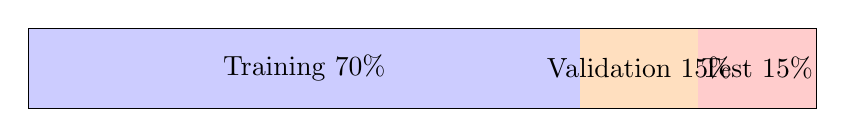
\begin{tikzpicture}[scale=1.0]
    \draw[thick] (0,0) rectangle (10,1);
    \fill[blue!20] (0,0) rectangle (7,1);
    \fill[orange!25] (7,0) rectangle (8.5,1);
    \fill[red!20] (8.5,0) rectangle (10,1);

    \node at (3.5,0.5) {Training 70\%};
    \node at (7.75,0.5) {Validation 15\%};
    \node at (9.25,0.5) {Test 15\%};
\end{tikzpicture}
\end{center}

\subsection{Vai trò của training set}

Training set là tập được dùng để cập nhật tham số của mô hình.

\[
    \text{Training set}
    \rightarrow
    \text{tính loss}
    \rightarrow
    \text{backpropagation}
    \rightarrow
    \text{cập nhật trọng số}
\]

\subsection{Vai trò của validation set}

Validation set không dùng để cập nhật trọng số trực tiếp. Nó được dùng để đánh giá mô hình trong quá trình huấn luyện.

Ta dùng validation set để:

\begin{itemize}
    \item theo dõi mô hình có overfit không;
    \item chọn mô hình tốt;
    \item điều chỉnh hyperparameter;
    \item quyết định thời điểm dừng huấn luyện.
\end{itemize}

\begin{ghinho}
Validation set được dùng trong quá trình huấn luyện để đánh giá và lựa chọn mô hình, nhưng không được dùng để cập nhật trọng số như training set.
\end{ghinho}

\subsection{Vai trò của test set}

Test set là tập dữ liệu chỉ dùng để đánh giá cuối cùng.

\begin{canhbao}
Test set không được dùng trong quá trình huấn luyện, không được dùng để chỉnh mô hình, không được dùng để chọn hyperparameter. Test set chỉ được dùng khi ta đã quyết định mô hình cuối cùng.
\end{canhbao}

\subsection{Ví dụ chia dữ liệu}

Giả sử có 1,000 ảnh.

Có thể chia:

\[
    700 \text{ ảnh training}
\]

\[
    150 \text{ ảnh validation}
\]

\[
    150 \text{ ảnh test}
\]

Trong quá trình làm mô hình:

\begin{itemize}
    \item dùng 700 ảnh training để học;
    \item dùng 150 ảnh validation để theo dõi và điều chỉnh;
    \item cất riêng 150 ảnh test, chỉ dùng cuối cùng.
\end{itemize}

% ==========================================================
\section{Nguyên tắc sử dụng Test Set}

\subsection{Không được dùng test set nhiều lần để chỉnh mô hình}

Một lỗi nghiêm trọng là:

\begin{enumerate}
    \item huấn luyện mô hình;
    \item đem test set ra đánh giá;
    \item thấy kết quả chưa tốt;
    \item quay lại chỉnh mô hình;
    \item lại đem cùng test set ra đánh giá;
    \item lặp lại nhiều lần.
\end{enumerate}

Cách làm này làm mô hình hoặc quá trình lựa chọn mô hình dần dần khớp với test set.

\begin{canhbao}
Nếu dùng test set nhiều lần để quyết định chỉnh mô hình, test set không còn là tập kiểm tra độc lập nữa. Kết quả báo cáo sau đó có thể đánh giá sai năng lực thật của mô hình.
\end{canhbao}

\subsection{Vì sao đây là lỗi nghiêm trọng?}

Test set có vai trò mô phỏng dữ liệu mới trong thực tế. Nếu ta liên tục nhìn vào test set để chỉnh mô hình, ta đã làm mất tính độc lập của nó.

Khi đó, kết quả trên test set không còn phản ánh khả năng tổng quát hóa thật.

\subsection{Liên hệ với nghiên cứu khoa học}

Trong nghiên cứu khoa học, nếu báo cáo kết quả trên một test set đã bị dùng nhiều lần để chỉnh mô hình, kết quả có thể gây hiểu lầm rằng mô hình tốt hơn thực tế.

Điều này có thể bị xem là sai nguyên tắc nghiên cứu, thậm chí là gian lận nếu cố ý.

\begin{ghinho}
Test set là bài kiểm tra cuối cùng. Nếu đã dùng test set để chỉnh mô hình, cần có một test set độc lập mới để đánh giá cuối cùng.
\end{ghinho}

\subsection{Nếu lỡ dùng test set thì làm sao?}

Nếu đã lỡ dùng test set trong quá trình phát triển mô hình, cách xử lý đúng là:

\begin{itemize}
    \item thu thập thêm dữ liệu mới để làm test set độc lập;
    \item hoặc chia lại dữ liệu và tạo một test set mới chưa từng dùng;
    \item báo cáo rõ quy trình đánh giá.
\end{itemize}

% ==========================================================
\section{Cross-validation}

\subsection{Ý tưởng}

Khi dữ liệu ít, việc tách riêng một test set cố định có thể làm lãng phí dữ liệu. Một hướng xử lý là kiểm tra chéo, tiếng Anh là \textit{cross-validation}.

Ý tưởng chung:

\begin{itemize}
    \item chia dữ liệu thành nhiều phần;
    \item mỗi lần dùng một phần khác nhau làm tập kiểm tra;
    \item huấn luyện và đánh giá nhiều lần;
    \item tổng hợp kết quả.
\end{itemize}

\subsection{Ví dụ K-fold cross-validation}

Giả sử chia dữ liệu thành 5 phần:

\[
    D_1,D_2,D_3,D_4,D_5
\]

Ta thực hiện 5 lần:

\begin{center}
\begin{tabular}{ccc}
\toprule
Lần & Dùng để train & Dùng để kiểm tra \\
\midrule
1 & $D_2,D_3,D_4,D_5$ & $D_1$ \\
2 & $D_1,D_3,D_4,D_5$ & $D_2$ \\
3 & $D_1,D_2,D_4,D_5$ & $D_3$ \\
4 & $D_1,D_2,D_3,D_5$ & $D_4$ \\
5 & $D_1,D_2,D_3,D_4$ & $D_5$ \\
\bottomrule
\end{tabular}
\end{center}

Sau đó lấy trung bình kết quả đánh giá.

\begin{luuy}
Trong transcript, cross-validation chỉ được nhắc như một hướng liên quan khi cần chia lại và đánh giá dữ liệu nhiều lần. Nội dung chi tiết về cross-validation có thể học sâu hơn ở phần machine learning.
\end{luuy}

% ==========================================================
\section{Early Stopping -- Early Stopping}

\subsection{Early stopping là gì?}

Early stopping, hay dừng sớm, là kỹ thuật dừng quá trình huấn luyện khi mô hình bắt đầu có dấu hiệu overfitting.

Ta theo dõi loss trên:

\begin{itemize}
    \item training set;
    \item validation set.
\end{itemize}

Thông thường, training loss sẽ giảm dần. Nhưng nếu validation loss giảm đến một mức nào đó rồi bắt đầu tăng trở lại, đó là dấu hiệu mô hình đang overfit.

\subsection{Minh họa}

\begin{center}
\begin{tikzpicture}[scale=1.0,>=Stealth]
    \draw[->] (0,0) -- (8,0) node[right] {Thời gian huấn luyện};
    \draw[->] (0,0) -- (0,5) node[above] {Loss};

    % training loss
    \draw[thick,blue,smooth] plot coordinates {
        (0.5,4.4) (1.2,3.6) (2.0,2.8) (3.0,2.1)
        (4.0,1.6) (5.0,1.25) (6.0,1.05) (7.2,0.9)
    };
    \node[blue] at (6.7,1.3) {training loss};

    % validation loss
    \draw[thick,red,smooth] plot coordinates {
        (0.5,4.5) (1.2,3.7) (2.0,2.9) (3.0,2.2)
        (4.0,1.8) (5.0,1.65) (6.0,1.85) (7.2,2.3)
    };
    \node[red] at (6.6,2.6) {validation loss};

    % early stop point
    \draw[dashed] (5.0,0) -- (5.0,1.65);
    \filldraw[black] (5.0,1.65) circle (2pt);
    \node[below] at (5.0,0) {dừng};

\end{tikzpicture}
\end{center}

\subsection{Ý nghĩa}

Giả sử ban đầu dự định huấn luyện 100,000 bước. Nhưng sau 70,000 bước, validation loss bắt đầu tăng, trong khi training loss vẫn giảm. Khi đó nên dừng huấn luyện và giữ mô hình tại thời điểm validation loss tốt nhất.

\begin{ghinho}
Early stopping giúp tránh tình trạng mô hình tiếp tục học quá sát training set sau khi đã đạt khả năng tổng quát hóa tốt nhất trên validation set.
\end{ghinho}

\subsection{Không phải cứ early stopping là mô hình tốt}

Dừng sớm chỉ giúp giảm overfitting. Nó không đảm bảo mô hình cuối cùng chắc chắn tốt.

Nếu mô hình quá yếu, dữ liệu sai, hoặc bài toán chưa được thiết kế đúng, early stopping vẫn không cứu được mô hình.

% ==========================================================
\section{Dropout -- Dropout}

\subsection{Dropout là gì?}

Dropout là kỹ thuật trong quá trình huấn luyện, tại mỗi thời điểm, ta ngẫu nhiên loại bỏ một số neuron khỏi mạng với một xác suất nào đó.

Ví dụ, nếu xác suất giữ lại neuron là:

\[
    p = 0.5
\]

thì trung bình khoảng một nửa số neuron được giữ lại, một nửa bị tạm thời bỏ qua trong bước huấn luyện đó.

\begin{ghinho}
Dropout chỉ dùng trong quá trình training. Khi test hoặc sử dụng mô hình thật, ta dùng toàn bộ mạng.
\end{ghinho}

\subsection{Một thời điểm trong dropout là gì?}

Trong bài học, một ``thời điểm'' có thể hiểu là một lần đưa một mẫu dữ liệu vào mạng.

Ví dụ:

\begin{itemize}
    \item đưa ảnh thứ nhất vào, dropout một số neuron, tính xuôi, tính ngược, cập nhật;
    \item đưa ảnh thứ hai vào, dropout một nhóm neuron khác, tính xuôi, tính ngược, cập nhật;
    \item tiếp tục như vậy cho các mẫu tiếp theo.
\end{itemize}

\subsection{Minh họa dropout}

\begin{center}
\begin{tikzpicture}[x=2cm,y=1cm,>=Stealth,
    neuron/.style={circle,draw,minimum size=8mm},
    dropped/.style={circle,draw,dashed,gray,minimum size=8mm},
    every node/.style={font=\small}
]

% Input
\node[neuron] (i1) at (0,1) {$x_1$};
\node[neuron] (i2) at (0,0) {$x_2$};
\node[neuron] (i3) at (0,-1) {$x_3$};

% Hidden
\node[neuron] (h1) at (1.8,1.5) {$h_1$};
\node[dropped] (h2) at (1.8,0.5) {$h_2$};
\node[neuron] (h3) at (1.8,-0.5) {$h_3$};
\node[dropped] (h4) at (1.8,-1.5) {$h_4$};

% Output
\node[neuron] (o1) at (3.6,0.5) {$o_1$};
\node[neuron] (o2) at (3.6,-0.5) {$o_2$};

% Connections only active
\foreach \i in {i1,i2,i3}
    \foreach \h in {h1,h3}
        \draw[->] (\i) -- (\h);

\foreach \h in {h1,h3}
    \foreach \o in {o1,o2}
        \draw[->] (\h) -- (\o);

\node[gray] at (1.8,-2.1) {Neuron nét đứt bị dropout};

\end{tikzpicture}
\end{center}

\subsection{Vì sao dropout giúp giảm overfitting?}

Có hai cách hiểu trực quan.

\subsection{Góc nhìn ensemble}

Nếu mỗi lần dropout tạo ra một cấu hình mạng khác nhau, thì trong quá trình huấn luyện, ta giống như đang huấn luyện rất nhiều mạng con khác nhau.

Khi test, ta dùng toàn bộ mạng, có thể xem như sự kết hợp của nhiều mạng con đã được huấn luyện.

\begin{vidu}
Thay vì huấn luyện một mạng duy nhất, dropout khiến mô hình trải qua rất nhiều phiên bản mạng con. Điều này gần giống tư tưởng ensemble: nhiều mô hình cùng đóng góp để tạo ra kết quả ổn định hơn.
\end{vidu}

\subsection{Góc nhìn giảm phụ thuộc}

Nếu không có dropout, một neuron có thể phụ thuộc quá mạnh vào một vài neuron khác. Khi dropout ngẫu nhiên loại bỏ neuron, mạng buộc phải học cách sử dụng thông tin từ nhiều nguồn khác nhau.

Điều này giúp mạng mạnh mẽ hơn và ít phụ thuộc vào một đường truyền thông tin cụ thể.

\begin{ghinho}
Dropout buộc các neuron phải ``học cách làm việc với nhiều đồng đội khác nhau'', thay vì phụ thuộc quá mức vào một vài neuron cố định.
\end{ghinho}

\subsection{Dropout và robust model}

Một mô hình robust là mô hình vẫn hoạt động tốt trong nhiều tình huống khác nhau.

Dropout giúp tăng tính robust vì trong quá trình train, mạng thường xuyên phải làm việc trong điều kiện thiếu một số neuron. Nhờ đó, mạng học được biểu diễn phân tán hơn và ít nhạy với từng neuron riêng lẻ.

\subsection{Vì sao không dùng dropout khi test?}

Trong training, mỗi lần chỉ một phần neuron hoạt động. Nhưng khi test, ta muốn dùng toàn bộ năng lực của mạng đã học.

Vì vậy:

\[
    \text{Training: dùng dropout}
\]

\[
    \text{Testing: không dùng dropout}
\]

\subsection{Vấn đề scale tín hiệu}

Giả sử trong training, mỗi neuron được giữ lại với xác suất:

\[
    p=0.5
\]

Khi đó, trung bình một neuron ở lớp sau chỉ nhận được khoảng một nửa số tín hiệu so với khi dùng toàn bộ mạng.

Nếu khi test ta bật toàn bộ neuron mà không điều chỉnh gì, tổng tín hiệu đầu vào có thể tăng lên so với lúc training.

Theo cách trình bày trong bài học, để làm cho mức tín hiệu giữa training và testing tương thích hơn, output của neuron có thể được nhân với hệ số $p$ khi dùng toàn bộ mạng.

\[
    out_{\text{test}} = p \cdot out
\]

Ví dụ nếu:

\[
    p=0.5
\]

thì khi test:

\[
    out_{\text{test}}=0.5\cdot out
\]

\begin{luuy}
Trong nhiều thư viện hiện đại, người ta thường dùng biến thể gọi là inverted dropout: scale ngay trong lúc training, nên khi test không cần nhân thêm. Ý chính cần nhớ trong bài này là phải giữ mức tín hiệu giữa training và testing nhất quán.
\end{luuy}

\subsection{Xác suất dropout}

Giá trị $p$ là một hyperparameter. Ví dụ phổ biến:

\[
    p=0.5
\]

Nhưng không có một giá trị tốt nhất cho mọi bài toán. Trong thực tế, người ta thường dùng các giá trị đã được nghiên cứu trước hoặc thử nghiệm để chọn giá trị phù hợp.

\begin{luuy}
Không nên hiểu rằng $p=0.5$ luôn là tốt nhất. Nó chỉ là một lựa chọn phổ biến trong nhiều tình huống.
\end{luuy}

% ==========================================================
\section{Tổng hợp các kỹ thuật xử lý Overfitting}

\subsection{Các kỹ thuật chính}

\begin{center}
\begin{tabular}{p{0.28\textwidth}p{0.60\textwidth}}
\toprule
Kỹ thuật & Ý nghĩa \\
\midrule
Đơn giản hóa mô hình & Giảm số lớp, số neuron hoặc độ phức tạp để tránh học nhiễu \\
Feature selection & Bỏ bớt đặc trưng không cần thiết hoặc gây nhiễu \\
Thêm dữ liệu & Thu thập thêm dữ liệu thật, độc lập và đa dạng \\
Data augmentation & Tạo thêm dữ liệu hợp lý từ dữ liệu gốc \\
Train/validation/test split & Đánh giá đúng khả năng tổng quát hóa \\
Early stopping & Dừng khi validation loss bắt đầu xấu đi \\
Dropout & Ngẫu nhiên loại neuron trong training để giảm phụ thuộc và tăng robust \\
Cross-validation & Đánh giá ổn định hơn khi dữ liệu ít \\
\bottomrule
\end{tabular}
\end{center}

\subsection{Kỹ thuật nào quan trọng nhất?}

Không có một kỹ thuật duy nhất giải quyết mọi trường hợp. Trong thực tế thường phải kết hợp nhiều kỹ thuật.

Ví dụ với bài toán ảnh:

\begin{itemize}
    \item dùng mô hình đủ mạnh;
    \item dùng data augmentation;
    \item chia train/validation/test đúng;
    \item theo dõi validation loss;
    \item dùng early stopping;
    \item dùng dropout hoặc các kỹ thuật regularization khác.
\end{itemize}

% ==========================================================
\section{Technical Glossary -- Bảng thuật ngữ chuyên ngành}

\small
\begin{longtable}{p{0.26\textwidth}p{0.48\textwidth}p{0.19\textwidth}}
\toprule
\textbf{Thuật ngữ} & \textbf{Giải thích} & \textbf{Ví dụ} \\
\midrule
\endfirsthead

\toprule
\textbf{Thuật ngữ} & \textbf{Giải thích} & \textbf{Ví dụ} \\
\midrule
\endhead

Underfitting & Mô hình chưa khớp dữ liệu, chưa học được xu hướng tổng quát. & Dùng đường thẳng cho dữ liệu cong. \\

Overfitting & Mô hình quá khớp training data, học cả nhiễu. & Đa thức bậc cao đi qua mọi điểm. \\

Training set & Tập dữ liệu dùng để cập nhật tham số mô hình. & 70\% dữ liệu. \\

Validation set & Tập dùng để đánh giá trong quá trình huấn luyện và chọn mô hình. & 15\% dữ liệu. \\

Test set & Tập chỉ dùng để đánh giá cuối cùng. & 15\% dữ liệu còn lại. \\

Data augmentation & Tạo thêm dữ liệu từ dữ liệu gốc bằng biến đổi hợp lý. & Crop, flip, rotate ảnh. \\

Crop & Cắt một vùng trong ảnh gốc để tạo ảnh mới. & Cắt vùng chứa con chó. \\

Reflection/Flip & Lật ảnh theo chiều ngang hoặc chiều dọc. & Lật ảnh voi quay phải thành quay trái. \\

Rotation & Xoay ảnh một góc nào đó. & Xoay ảnh búa 30 độ. \\

Color augmentation & Thay đổi màu sắc, độ sáng hoặc kênh màu. & Làm ảnh hoa sáng hơn. \\

Early stopping & Dừng sớm khi validation loss bắt đầu tăng. & Dừng sau 5 ngày thay vì 7 ngày. \\

Dropout & Ngẫu nhiên loại bỏ một số neuron trong quá trình training. & Giữ lại neuron với xác suất 0.5. \\

Ensemble & Kết hợp nhiều mô hình để có kết quả ổn định hơn. & Trung bình kết quả nhiều mạng. \\

Robust & Mạnh mẽ, ít bị ảnh hưởng bởi thay đổi nhỏ hoặc thiếu một phần thông tin. & Mạng không phụ thuộc một neuron. \\

Hyperparameter & Tham số do người thiết kế chọn trước hoặc điều chỉnh. & Dropout rate, số lớp. \\

Cross-validation & Kiểm tra chéo, chia dữ liệu nhiều lần để đánh giá ổn định hơn. & 5-fold cross-validation. \\

Feature selection & Chọn hoặc loại bỏ đặc trưng đầu vào. & Bỏ chỉ số không liên quan. \\

Generalization & Khả năng tổng quát hóa trên dữ liệu mới. & Test accuracy cao. \\

\bottomrule
\end{longtable}
\normalsize

% ==========================================================
\section{Key Concepts Summary -- Tóm tắt kiến thức trọng tâm}

\subsection{Các ý chính cần nhớ}

\begin{enumerate}
    \item Underfitting xảy ra khi mô hình quá đơn giản hoặc chưa được huấn luyện đủ.
    \item Overfitting xảy ra khi mô hình quá phức tạp, dữ liệu ít hoặc thiếu đa dạng.
    \item Underfitting dễ nhận ra hơn vì loss thường còn cao.
    \item Overfitting nguy hiểm hơn vì training loss thấp khiến ta dễ nhầm rằng mô hình tốt.
    \item Để giảm underfitting, có thể dùng mô hình mạnh hơn hoặc huấn luyện lâu hơn.
    \item Để giảm overfitting, có thể đơn giản hóa mô hình, bỏ bớt đặc trưng, thêm dữ liệu hoặc dùng data augmentation.
    \item Data augmentation giúp tăng cả số lượng và độ đa dạng dữ liệu.
    \item Augmentation phải tạo ra dữ liệu hợp lý với bài toán thực tế.
    \item Dữ liệu nên được chia thành training, validation và test set.
    \item Test set chỉ được dùng để đánh giá cuối cùng.
    \item Dùng test set nhiều lần để chỉnh mô hình là sai nguyên tắc.
    \item Early stopping dùng validation loss để dừng trước khi mô hình overfit.
    \item Dropout ngẫu nhiên loại neuron trong training để giảm phụ thuộc và tăng khả năng tổng quát hóa.
    \item Dropout chỉ dùng trong training, không dùng trong testing.
\end{enumerate}

\subsection{Công thức và con số cần nhớ}

\subsection*{Tỷ lệ chia dữ liệu ví dụ}

\[
    70\% \text{ training}
    \quad
    15\% \text{ validation}
    \quad
    15\% \text{ test}
\]

\subsection*{Số ảnh trung bình mỗi class}

\[
    \frac{1,200,000}{1000}=1200 \text{ ảnh/class}
\]

\subsection*{Data augmentation 2048 lần}

\[
    1,200,000 \times 2048
    =
    2,457,600,000
\]

\[
    \approx 2.46 \text{ tỷ ảnh}
\]

\subsection*{Dropout scale theo xác suất giữ neuron}

\[
    out_{\text{test}} = p \cdot out
\]

% ==========================================================
\section{Review Questions -- Câu hỏi ôn tập}

\begin{enumerate}
    \item Underfitting là gì?
    \item Overfitting là gì?
    \item Vì sao overfitting nguy hiểm hơn underfitting trong quá trình đánh giá mô hình?
    \item Nêu hai nguyên nhân gây underfitting.
    \item Nêu ba nguyên nhân gây overfitting.
    \item Vì sao dữ liệu nhiều nhưng thiếu đa dạng vẫn có thể gây overfitting?
    \item Data augmentation là gì?
    \item Nêu ba kỹ thuật data augmentation cho ảnh.
    \item Vì sao không nên xoay ảnh một cách tùy tiện?
    \item Training set dùng để làm gì?
    \item Validation set dùng để làm gì?
    \item Test set dùng để làm gì?
    \item Vì sao không được dùng test set nhiều lần để chỉnh mô hình?
    \item Early stopping hoạt động dựa trên dấu hiệu nào?
    \item Dropout là gì?
    \item Dropout được dùng trong training hay testing?
    \item Vì sao dropout có thể giúp giảm overfitting?
    \item Xác suất giữ neuron $p=0.5$ có phải luôn là tốt nhất không?
\end{enumerate}

% ==========================================================
\section{Practice Exercises -- Bài tập vận dụng}

\subsection*{Bài tập 1: Nhận diện lỗi mô hình}
\addcontentsline{toc}{section}{Bài tập 1: Nhận diện lỗi mô hình}

Xác định trường hợp sau là underfitting hay overfitting:

\begin{enumerate}
    \item Training loss cao, validation loss cao.
    \item Training loss rất thấp, validation loss cao.
    \item Mô hình dùng đường thẳng cho dữ liệu có dạng cong.
    \item Mô hình dùng đa thức bậc rất cao và đi qua mọi điểm training.
\end{enumerate}

\subsection*{Lời giải gợi ý}

\begin{enumerate}
    \item Underfitting.
    \item Overfitting.
    \item Underfitting.
    \item Overfitting.
\end{enumerate}

\subsection*{Bài tập 2: Chia dữ liệu}
\addcontentsline{toc}{section}{Bài tập 2: Chia dữ liệu}

Bạn có 10,000 ảnh. Hãy chia theo tỷ lệ:

\[
    70\% \text{ training}, \quad 15\% \text{ validation}, \quad 15\% \text{ test}
\]

Tính số ảnh trong mỗi tập.

\subsection*{Lời giải gợi ý}

Training:

\[
    10,000 \times 0.70 = 7,000
\]

Validation:

\[
    10,000 \times 0.15 = 1,500
\]

Test:

\[
    10,000 \times 0.15 = 1,500
\]

\subsection*{Bài tập 3: Data augmentation}
\addcontentsline{toc}{section}{Bài tập 3: Data augmentation}

Một tập dữ liệu có 5,000 ảnh. Nếu mỗi ảnh được augmentation thành 100 ảnh, tổng số ảnh sau augmentation là bao nhiêu?

\subsection*{Lời giải gợi ý}

\[
    5,000 \times 100 = 500,000
\]

Vậy sau augmentation có 500,000 ảnh.

\subsection*{Bài tập 4: Chọn augmentation phù hợp}
\addcontentsline{toc}{section}{Bài tập 4: Chọn augmentation phù hợp}

Với từng bài toán, hãy cho biết phép augmentation nào hợp lý hơn:

\begin{enumerate}
    \item Nhận dạng cây búa trong ảnh.
    \item Nhận dạng ngôi nhà bình thường.
    \item Nhận dạng hoa hồng trong nhiều điều kiện ánh sáng.
    \item Nhận dạng con voi trong ảnh tự nhiên.
\end{enumerate}

\subsection*{Lời giải gợi ý}

\begin{enumerate}
    \item Có thể xoay ảnh nhiều góc nếu cây búa có thể xuất hiện ở nhiều hướng.
    \item Có thể crop, đổi sáng, xoay nhẹ; không nên lật ngược nhà 180 độ nếu thực tế không có nhà lộn ngược.
    \item Nên đổi sáng, màu sắc, tương phản.
    \item Có thể crop, lật ngang, xoay nhẹ; không nên lật ngược voi nếu bài toán không có tình huống đó.
\end{enumerate}

\subsection*{Bài tập 5: Dropout}
\addcontentsline{toc}{section}{Bài tập 5: Dropout}

Một layer có 100 neuron. Nếu dùng dropout với xác suất giữ lại:

\[
    p=0.5
\]

Trung bình mỗi lần training có bao nhiêu neuron được giữ lại?

\subsection*{Lời giải gợi ý}

\[
    100 \times 0.5 = 50
\]

Trung bình có 50 neuron được giữ lại.

% ==========================================================
\section*{Kết luận}
\addcontentsline{toc}{section}{Kết luận}

ANN8 giải thích sâu hơn nguyên nhân và cách xử lý underfitting, overfitting. Underfitting thường xảy ra khi mô hình quá đơn giản hoặc chưa được huấn luyện đủ. Overfitting thường xảy ra khi mô hình quá phức tạp, dữ liệu quá ít hoặc thiếu đa dạng.

Để xử lý underfitting, ta có thể dùng mô hình mạnh hơn hoặc huấn luyện lâu hơn. Để xử lý overfitting, ta có nhiều kỹ thuật như đơn giản hóa mô hình, bỏ bớt đặc trưng, tăng dữ liệu, data augmentation, chia đúng train/validation/test, early stopping và dropout.

Một điểm rất quan trọng của bài học là nguyên tắc sử dụng test set. Test set chỉ dùng để đánh giá cuối cùng, không dùng để chỉnh mô hình. Nếu dùng test set nhiều lần trong quá trình phát triển, kết quả đánh giá cuối cùng sẽ không còn đáng tin cậy.

Cuối cùng, dropout được trình bày như một kỹ thuật rất phổ biến để giảm overfitting. Nó ngẫu nhiên loại bỏ neuron trong quá trình training, buộc mạng học biểu diễn mạnh mẽ hơn và ít phụ thuộc vào một số neuron cụ thể.

